\documentclass[12pt]{article}

\usepackage{amsmath, mathtools}
\usepackage{amsfonts}
\usepackage{amssymb}
\usepackage{graphicx}
\usepackage{colortbl}
\usepackage{xr}
\usepackage{hyperref}
\usepackage{longtable}
\usepackage{xfrac}
\usepackage{tabularx}
\usepackage{float}
\usepackage{siunitx}
\usepackage{booktabs}
\usepackage{caption}
\usepackage{pdflscape}
\usepackage{afterpage}

\usepackage[round]{natbib}

%\usepackage{refcheck}

\hypersetup{
   % bookmarks=true,         % show bookmarks bar?
      colorlinks=true,       % false: boxed links; true: colored links
    linkcolor=red,          % color of internal links (change box color with linkbordercolor)
    citecolor=green,        % color of links to bibliography
    filecolor=magenta,      % color of file links
    urlcolor=cyan           % color of external links
}

%% Comments

\usepackage{color}

\newif\ifcomments\commentstrue

\ifcomments
\newcommand{\authornote}[3]{\textcolor{#1}{[#3 ---#2]}}
\newcommand{\todo}[1]{\textcolor{red}{[TODO: #1]}}
\else
\newcommand{\authornote}[3]{}
\newcommand{\todo}[1]{}
\fi

\newcommand{\wss}[1]{\authornote{blue}{SS}{#1}}
\newcommand{\an}[1]{\authornote{magenta}{Author}{#1}}



% For easy change of table widths
\newcommand{\colZwidth}{1.0\textwidth}
\newcommand{\colAwidth}{0.13\textwidth}
\newcommand{\colBwidth}{0.82\textwidth}
\newcommand{\colCwidth}{0.1\textwidth}
\newcommand{\colDwidth}{0.05\textwidth}
\newcommand{\colEwidth}{0.8\textwidth}
\newcommand{\colFwidth}{0.17\textwidth}
\newcommand{\colGwidth}{0.5\textwidth}
\newcommand{\colHwidth}{0.28\textwidth}

% Used so that cross-references have a meaningful prefix
\newcounter{defnum} %Definition Number
\newcommand{\dthedefnum}{GD\thedefnum}
\newcommand{\dref}[1]{GD\ref{#1}}
\newcounter{datadefnum} %Datadefinition Number
\newcommand{\ddthedatadefnum}{DD\thedatadefnum}
\newcommand{\ddref}[1]{DD\ref{#1}}
\newcounter{theorynum} %Theory Number
\newcommand{\tthetheorynum}{T\thetheorynum}
\newcommand{\tref}[1]{T\ref{#1}}
\newcounter{tablenum} %Table Number
\newcommand{\tbthetablenum}{T\thetablenum}
\newcommand{\tbref}[1]{TB\ref{#1}}
\newcounter{assumpnum} %Assumption Number
\newcommand{\atheassumpnum}{P\theassumpnum}
\newcommand{\aref}[1]{A\ref{#1}}
\newcounter{goalnum} %Goal Number
\newcommand{\gthegoalnum}{P\thegoalnum}
\newcommand{\gsref}[1]{GS\ref{#1}}
\newcounter{instnum} %Instance Number
\newcommand{\itheinstnum}{IM\theinstnum}
\newcommand{\iref}[1]{IM\ref{#1}}
\newcounter{reqnum} %Requirement Number
\newcommand{\rthereqnum}{P\thereqnum}
\newcommand{\rref}[1]{R\ref{#1}}
\newcounter{lcnum} %Likely change number
\newcommand{\lthelcnum}{LC\thelcnum}
\newcommand{\lcref}[1]{LC\ref{#1}}

\newcommand{\progname}{ProgName} % PUT YOUR PROGRAM NAME HERE

\usepackage{fullpage}

\begin{document}

\title{CAS 741: SRS \\A numerical search for the spectrum related to travelling 
periodic waves} 
\author{Robert White}
\date{\today}
	
\maketitle

~\newpage

\pagenumbering{roman}

\section{Revision History}

\begin{tabularx}{\textwidth}{p{3cm}p{2cm}X}
\toprule {\bf Date} & {\bf Version} & {\bf Notes}\\
\midrule
25-09-2018 & 1.0 & Creation of first draft\\
29-09-2018 & 1.1 & Edit of 1.1. Added a GS, responsibilites, requirenments, 
definitions and verification of compatibility. Updated comments .tex. My 
comments are in red, SS comments are in blue.\\
\bottomrule
\end{tabularx}

~\newpage

\section{Reference Material}

This section records information for easy reference.

\subsection{Table of Units}

Throughout this document SI (Syst\`{e}me International d'Unit\'{e}s) is employed
as the unit system.  In addition to the basic units, several derived units are
used as described below.  For each unit, the symbol is given followed by a
description of the unit and the SI name. \\
\wrw{Is it OK if we mark some units as unitless? My supervisor and I are more 
concerned about mathematical properties, not physical.}
~\newline

\renewcommand{\arraystretch}{1.2}
%\begin{table}[ht]
  \noindent \begin{tabular}{l l l} 
    \toprule		
    \textbf{symbol} & \textbf{unit} & \textbf{SI}\\
    \midrule 
    \si{\metre} & length & metre\\
    t & time & second\\
    \bottomrule
  \end{tabular}
  %	\caption{Provide a caption}
%\end{table}


\subsection{Table of Symbols}

The table that follows summarizes the symbols used in this document along with
their units.  The choice of symbols was made to be consistent with the heat
transfer literature and with existing documentation for solar water heating
systems.  The symbols are listed in alphabetical order.

\renewcommand{\arraystretch}{1.2}
%\noindent \begin{tabularx}{1.0\textwidth}{l l X}
\noindent \begin{longtable*}{l l p{12cm}} \toprule
\textbf{symbol} & \textbf{unit} & \textbf{description}\\
\midrule 
$\lambda$ &  & spectral parameter
\\
$u$ &  & wave amplitude 
\\  
$\phi$ & & eigen function
\\ 
$c$ & & wave speed 
\\
$\omega$ & & angular frequency 
\\ 
\bottomrule
\end{longtable*}

\subsection{Abbreviations and Acronyms}

\renewcommand{\arraystretch}{1.2}
\begin{tabular}{l l} 
  \toprule		
  \textbf{symbol} & \textbf{description}\\
  \midrule 
  A & Assumption\\
  $\mathbb{C}$ & Complex numbers\\
  cn & Elliptic cosine \\
  DD & Data Definition\\
  dn & Delta amplitude \\
  GD & General Definition\\
  GS & Goal Statement\\
  $i$ & imaginary number\\
  IM & Instance Model\\
  LC & Likely Change\\
  NLS & Nonlinear Schrodinger\\
  ODE & Ordinary Differential Equation\\
  PDE & Partial Differential Equation\\
  PS & Physical System Description\\
  $\mathbb{R}$ & Real number line\\
  R & Requirement\\ 
  sn & Elliptic sine\\
  SRS & Software Requirements Specification\\
  \progname{} & SpecSearch\\
  T & Theoretical Model\\  
  \bottomrule
\end{tabular}\\

\subsection{Mathematical Notation}
Let $u$ be a complex number of the form $u= m + ni$, where $m,n \in 
\mathbb{R}$. The complex conjugate of $u$ is defined to be $\bar{u}= m - ni$. 
The modulus of $u$ is defined to be $|u| = \sqrt{m^{2}+n^{2}}$. \\

Let $u(x,t): \mathbb{R}^{2} -> \mathbb{C}$. We will let $u_{t}$ denote the 
partial derivative of $u$ with respect to t. Similarily, $u_{x}$ is the partial 
derivative of u with respect to x. If $u$ has a one independent variable than 
we will denote its derivative by $u'$. \\

\wrw{Why is this section before the table of contents?}

\newpage

\tableofcontents

~\newpage

\pagenumbering{arabic}

\section{Introduction}

\subsection{Purpose of Document}
The purpose of this document is to describe the requirements for the spectral 
search program. The spectral search program will search for the location of the 
continuous spectrum of a particular lax equation related to the NLS equation. 
This abstract document will explain the mathematical models, assumptions, 
solution characterisitcs and goals of the software. After reading this doucment 
one should be able to understand the mathematical and physical context of the 
inputs and outputs. They should also be able to identify the constraints of the 
system and have an idea as to how the output is derived from the given input.  
The SRS is meant to be unambigious and will not provide a detailed explanation 
of the numerical solution or code. \\
The SRS details the quality attributes of the software, such as functionality, 
without dicussing any code, numerical algorithms or scientific computing 
solutions. It is a precursor to the documents required in the development of 
scientific software. One should read and understand this document before the 
VnV, design or code itself. \\


\subsection{Scope of Requirements} 

The scope of SpecSearch is limited to the creation of a spectral diagram for a 
particular linear lax equation. The waves being investigated are solutions to 
the NLS equation. The spectrum will be plotted on the complex plane. 

\subsection{Characteristics of Intended Reader} 

The intended reader of this document should have taken an introductory course 
in partial differential equations and complex analysis. They should also have a 
first year undergraduate understanding of linear algebra.\\

\subsection{Organization of Document}

This document follows a template provided by Dr. Spencer Smith at McMaster 
University. It begins by introducing the document. This intdocution is followed 
by a general overview of the system and than an outline of the goals and 
mathematical theory. The document continues with behaviour between inputs and 
outputs, judging output and than foreshadows changes to the software. It 
concludes with useful graphs. \\ 
More details of the template can be found in Smith et al (2005) and Smith et al 
(2007). The latex template is available in Dr. Spencer Smith's gitlab 
repository CAS 741. \\

\section{General System Description}

This section identifies the interfaces between the system and its environment,
describes the user characteristics and lists the system constraints.

\subsection{System Context}

\begin{itemize}
\item User Responsibilities:
\begin{itemize}
\item Ensure that the input variables resemble the wave they intend to analyze.
\item Ensure that the assumptions imposed on waves in this model are reasonable 
for the user's reasearch
\item Understand research limitations of software model, such as strict 
assumptions on physical system.
\end{itemize}
\item \progname{} Responsibilities:
\wrw{I am wondering if my responsibilities are similar to Goal Statements and 
functional requirenments..}
\begin{itemize}
\item Detect data type mismatch. 
\item Solve the lax equation associated with given wave parameters. 
\item Connect the discrete spectrum in order to form a continuous spectrum. 
\item Plot the continuous spectrum on the complex plane.
\item Determine whether or not the solution is stable. 
\end{itemize}
\end{itemize}

\subsection{User Characteristics} \label{SecUserCharacteristics}

The end user of SpecSearch should have an introductory level understanding of 
complex analysis and partial differential equations. They should also be 
familiar with matrix alegbra and eigenvectors presented in a first year course 
in linear algebra. 

\subsection{System Constraints}

The system only deals with general traveling periodic wave solutions of the 
NLS. 

\section{Specific System Description}

This section first presents the problem description, which gives a high-level
view of the problem to be solved.  This is followed by the solution 
characteristics specification, which presents the assumptions, theories, 
definitions and finally the instance models. 

\subsection{Problem Description} \label{Sec_pd}
A lax pair is a set of matrices or operators that satisfy differential 
equations. The NLS equation, a PDE used to model rogue waves and modulated wave 
packets, appears as a compatibility condition of a particular lax pair of 
equations. One equation is a spectral problem and the other is a time 
evolution problem.  \\

SpecSearch will produce a graph of a numerical approximation of the continuous 
spectrum of a lax linear equation assocaited with general travelling periodic 
wave solutions of the NLS equation. Previous attempts have used an algebraic 
method to calculate the spectral parameter. These attempts have only been 
successful at finding a countable number of eigenvalues. This software will 
"connect" these points in an attempt to approximate and search for the 
continuous spectrum. \\ 

\subsubsection{Terminology and  Definitions}

This subsection provides a list of terms that are used in the subsequent
sections and their meaning, with the purpose of reducing ambiguity and making it
easier to correctly understand the requirements:

\begin{itemize}

\item \textbf{Spectrum}: The set of allowable values for the spectral parameter 
of a matrix or operator.
\item \textbf{Operator}: A mapping that transforms elements of a space int 
other elements of the same space. 
\item \textbf{Traveling Periodic Wave}: A periodic and one-dimensional wave 
that travels with a constant speed. 
\item \textbf{Compatibility Condition}: Conditions under which the lax pair of 
equations is guaranteed. 
\item \textbf{Stability}: A solution is stable if it slight perturbations lead 
to at most slight perturbations in the solution.
\item \textbf{Initial Data}: The initial profile of a wave (or its derivative) 
at a fixed point in time.
\item \textbf{Rogue Wave}: A wave is considered rogue if its amplitude is more 
than double of the average of the upper third surrounding wave amplitudes.

\end{itemize}

\subsubsection{Physical System Description}

The physical system of SpecSearch includes the following elements:

\begin{itemize}

\item[PS\refstepcounter{goalnum}\thegoalnum \label{G_meaningfulLabel}:] 
Unspecified body of water or laser channel with a traveling periodic 
wave.

\end{itemize}

\subsubsection{Goal Statements}
\wrw{Are these too similar to functional responsibilities and requirenments?}
\noindent Given the constant wave speed, c , angular frequenct ,$\omega$, and 
intial profile of a general traveling periodic wave, the goal statements are:

\begin{itemize}

\item[GS\refstepcounter{goalnum}\thegoalnum \label{G_meaningfulLabel}:] 
Find elements of the continuous spectrum on the complex plane for a general 
traveling periodic wave. 
\item[GS\refstepcounter{goalnum}\thegoalnum \label{G_meaningfulLabel}:] 
Approximate the coninuous spectrum given the points from GS1.
\item[GS\refstepcounter{goalnum}\thegoalnum \label{G_meaningfulLabel}:] 
Determine the stability of traveling wave solutions.

\end{itemize}

\subsection{Solution Characteristics Specification}

The instance models that govern SpecSearch are presented in
Subsection~\ref{sec_instance}.  The information to understand the meaning of the
instance models and their derivation is also presented, so that the instance
models can be verified.

\subsubsection{Assumptions}

This section simplifies the original problem and helps in developing the
theoretical model by filling in the missing information for the physical
system. The numbers given in the square brackets refer to the theoretical model
[T], general definition [GD], data definition [DD], instance model [IM], or
likely change [LC], in which the respective assumption is used.

\begin{itemize}

\item[A\refstepcounter{assumpnum}\theassumpnum \label{A_meaningfulLabel}:]The 
wave equation is a complex hamiltonian evolution equation. 
\item[A\refstepcounter{assumpnum}\theassumpnum \label{A_meaningfulLabel}:]The 
linear momentum densities are proportional to the integrands of the 
corresponding velocity functionals 
\item[A\refstepcounter{assumpnum}\theassumpnum \label{A_meaningfulLabel}:]All 
waves in the model are general traveling perioidic waves with constant speed 
and frequency. 
\item[A\refstepcounter{assumpnum}\theassumpnum \label{A_meaningfulLabel}:]The 
wave is a solution to the NLS equation.
\item[A\refstepcounter{assumpnum}\theassumpnum \label{A_meaningfulLabel}:]The 
system only deals with focusing waves.

\end{itemize}

\subsubsection{Theoretical Models}\label{sec_theoretical}

This section focuses on the general equations and laws that SpecSearch is based
on. 

~\newline

\noindent
\begin{minipage}{\textwidth}
\renewcommand*{\arraystretch}{1.5}
\begin{tabular}{| p{\colAwidth} | p{\colBwidth}|}
  \hline
  \rowcolor[gray]{0.9}
  Number& T\refstepcounter{theorynum}\thetheorynum \label{T_COE}\\
  \hline
  Label&\bf Nonlinear focusing shchrodinger equation\\
  \hline
  Equation&  $ iu_{t} + u_{xx} + 2|u|^{2}u=0$\\
  \hline
  Description & 
                The above equation is a PDE meant to model modulated wave 
                packets and rogue waves in physics. $u$ is the complex envelope 
                of the wave, $t$ is time and $x$ is the position in one 
                dimensional space.\\
  \hline
  Source &
           \url{http://www.efunda.com/formulae/heat_transfer/conduction/overview_cond.cfm}\\
  % The above web link should be replaced with a proper citation to a publication
  \hline
  Ref.\ By & \dref{ROCT}\\
  \hline
\end{tabular}
\end{minipage}\\

~\newline



\subsubsection{General Definitions}\label{sec_gendef}

This section collects the laws and equations that will be used in deriving the
data definitions, which in turn are used to build the instance models.
\wrw{Should T2 be a data definition?}
~\newline
\noindent
\begin{minipage}{\textwidth}
	\renewcommand*{\arraystretch}{1.5}
	\begin{tabular}{| p{\colAwidth} | p{\colBwidth}|}
		\hline
		\rowcolor[gray]{0.9}
		Number& T\refstepcounter{theorynum}\thetheorynum \label{T_COE}\\
		\hline
		Label&\bf General travelling periodic wave\\
		\hline
		Equation&  $ u(x,t)=u(x+2ct)e^{i\omega t}$\\
		\hline
		Description & 
		This is the standard form of a traveling periodic wave. The variables 
		$c$ and $\omega$ denote the wave speed and angular frequency 
		respectively. $u(x+2ct)$ represents an amplitude value traveling in 
		time for a fixed x value.\\
		\hline
		Source &
		\url{http://www.efunda.com/formulae/heat_transfer/conduction/overview_cond.cfm}\\
		% The above web link should be replaced with a proper citation to a 
		%publication
		\hline
		Ref.\ By & \dref{ROCT}\\
		\hline
	\end{tabular}
\end{minipage}\\

~\newline

\noindent
\begin{minipage}{\textwidth}
	\renewcommand*{\arraystretch}{1.5}
	\begin{tabular}{| p{\colAwidth} | p{\colBwidth}|}
		\hline
		\rowcolor[gray]{0.9}
		Number& T\refstepcounter{theorynum}\thetheorynum \label{T_COE}\\
		\hline
		Label&\bf General travelling periodic wave\\
		\hline
		Equation&  $ u'' + 2|u|^{2}u+2icu'=\omega u$\\
		\hline
		Description & 
		A reduction of T1 into a second order ODE. This is derived by 
		substituting T2 into T1. \\
		\hline
		Source &
		\url{http://www.efunda.com/formulae/heat_transfer/conduction/overview_cond.cfm}\\
		% The above web link should be replaced with a proper citation to a 
		%publication
		\hline
		Ref.\ By & T1,T2\\
		\hline
	\end{tabular}
\end{minipage}\\

~\newline

\subsubsection{Data Definitions}\label{sec_datadef}

This section collects and defines all the data needed to build the instance
models. The dimension of each quantity is also given. 
~\newline

\noindent
\begin{minipage}{\textwidth}
\renewcommand*{\arraystretch}{1.5}
\begin{tabular}{| p{\colAwidth} | p{\colBwidth}|}
\hline
\rowcolor[gray]{0.9}
Number& DD\refstepcounter{datadefnum}\thedatadefnum \label{FluxCoil}\\
\hline
Label& \bf Conservation Equations\\
\hline
Symbols &$g, c, d, \omega$\\
\hline
% Units& $Mt^{-3}$\\
% \hline
  SI Units & \si{\watt\per\square\metre}\\
  \hline
  Equation(1)&$\bar{u}u' - u\bar{u}' + 2ic|u|^{2} = 2ig$\\
  Equation(2)&$|u'|^{2} + |u|^{4} + d = \omega |u|^{2}$\\
  \hline
  Description & 
                Equation 1 (2) is derived by multiplying T3 by $\bar{u}$ 
                $(\bar{u}')$ and than subtracting (adding) the conjugate 
                equation. The resultant equations are integrated to yield 1 and 
                2.
  \\
  \hline
  Sources& Citation here \\
  \hline
  Ref.\ By & \iref{ewat}\\
  \hline
\end{tabular}
\end{minipage}\\

\subsubsection{Instance Models} \label{sec_instance}    

This section transforms the problem defined in Section~\ref{Sec_pd} into 
one which is expressed in mathematical terms. It uses concrete symbols defined 
in Section~\ref{sec_datadef} to replace the abstract symbols in the models 
identified in Sections~\ref{sec_theoretical} and~\ref{sec_gendef}.

The goals \wss{reference your goals} are solved by \wss{reference your instance
  models}.  \wss{other details, with cross-references where appropriate.}
\wss{Modify the examples below for your problem, and add additional models as
  appropriate.}

~\newline

%Instance Model 1

\noindent
\begin{minipage}{\textwidth}
\renewcommand*{\arraystretch}{1.5}
\begin{tabular}{| p{\colAwidth} | p{\colBwidth}|}
  \hline
  \rowcolor[gray]{0.9}
  Number& IM\refstepcounter{instnum}\theinstnum \label{ewat}\\
  \hline
  Label& \bf Searching for the continuous spectrum\\
  \hline
  Input&$c, \omega, g, d$, initial wave profile\\
  \hline
  Output&$\lambda$ such that:\\
  &$\phi_x = U(u,\lambda) \phi$\\
  \hline
  Description& $U(u,\lambda) = \begin{pmatrix} 
  \lambda & u \\
  -\bar{u} &-\lambda 
  \end{pmatrix}$ \\
  &T3 is a compabililty condition for the lax pair comprised of the above row's 
  ODE and $\phi_{t}=V(u,\lambda)\phi$\\
  &$V(u,\lambda)=\begin{pmatrix} 
  2 \lambda^{2} + |u|^{2} & u_{x}+2 \lambda u \\
  \bar{u}_{x}-2\lambda \bar{u} & -2\lambda^{2} - |u|^{2}
  \end{pmatrix}$ \\
  &$\phi \in \mathbb{C}$\\
  \hline
  Sources& Citation here \\
  \hline
  Ref.\ By & \iref{epcm}\\
  \hline
\end{tabular}
\end{minipage}\\
\newline \\
For a smooth $C^{2}$ function ,$\phi$, we have that $\phi_{tx}=\phi_{xt}$. \\
From IM1 $\Rightarrow \phi_{tx} = \delta_{t} U \phi + UV \phi$ and $\phi_{xt} = 
\delta_{x} V \phi + VU \phi$. \\
Combining the above two equations : \\
$\Rightarrow \delta_{t} U \phi + UV \phi = \delta_{x} V \phi + VU \phi$ \\
$\Rightarrow \delta_{t} U + UV = \delta_{x} V + VU$ (--) \\
Equating the two sides of (--) we arrive at 4 equalities (since each side is a 
2x2 
matrix) : \\
(1,1) : $ 0 + \lambda(-4\lambda^{3}-2\lambda u^{2}) + u(4\lambda^{2} u - 2 
\lambda u_{x} + 2 u^{3} + u_{xx}) = -4 \lambda u u_{x} + \lambda 
(-4\lambda^{3}-2\lambda u^{2} ) - u(-4\lambda^{2}u -2\lambda u_{x} - 2u^{3} 
-u_{xx})$ \\
$\Rightarrow 0=0$ \\ 
We have the same result for component (2,2) \\
(1,2) : $u_{t} + \lambda (-4\lambda^{2} u - 2\lambda u_{x} - 2u^{3} -u_{xx}) + 
u(4\lambda^{3}+2\lambda u^{2}) = -4\lambda^{2} u_{x} - 2\lambda u_{xx} - 
6u^{2}u_{x} - u_{xxx} + u(-4\lambda^{3} - 2\lambda u^{2}) - \lambda 
(-4\lambda^{2} u - 2\lambda u_{x} - 2u^{3} - u_{xx}) $ \\
$\Rightarrow u_{t} = -6u^{2}u_{x} - u_{xxx}$ $ \\
$$\Rightarrow u_{t} + 6u^{2}u_{x} + u_{xxx} = 0$ \\
The above equation is satisfied when $u$ is a solution to the NLS. \\
The result is the same for (2,1). Thus, the NLS is a compatability condition 
for IM1. 


\subsubsection{Data Constraints} \label{sec_DataConstraints}    

Tables~\ref{TblInputVar} and \ref{TblOutputVar} show the data constraints on the
input and output variables, respectively.  The column for physical constraints gives
the physical limitations on the range of values that can be taken by the
variable.  The column for software constraints restricts the range of inputs to
reasonable values.  The constraints are conservative, to give the user of the
model the flexibility to experiment with unusual situations.  The column of
typical values is intended to provide a feel for a common scenario.  The
uncertainty column provides an estimate of the confidence with which the
physical quantities can be measured.  This information would be part of the
input if one were performing an uncertainty quantification exercise.

The specification parameters in Table~\ref{TblInputVar} are listed in
Table~\ref{TblSpecParams}.

\begin{table}[!h]
\caption{Output Variables} \label{TblOutputVar}
\renewcommand{\arraystretch}{1.2}
\noindent \begin{longtable*}{l l} 
  \toprule
  \textbf{Var} & \textbf{Physical Constraints} \\
  \midrule 
  $\lambda$ & $\lambda \in \mathbb{C}$ 
  \\
  \bottomrule
\end{longtable*}
\end{table}

\subsubsection{Properties of a Correct Solution} \label{sec_CorrectSolution}

\noindent
A correct solution will be an array of numbers that appear on the continuous 
spectrum. The plot will connect these points in an attempt to model the entire 
continuous spectrum. The stability of solutions will be displayed as booleans. 

\section{Requirements}

This section provides the functional requirements, the business tasks that the
software is expected to complete, and the nonfunctional requirements, the
qualities that the software is expected to exhibit.\\

\wrw{Are these too similar to goal statements and responsibilites?}

\subsection{Functional Requirements}

\noindent \begin{itemize}

\item[R\refstepcounter{reqnum}\thereqnum \label{R_Inputs}:] SpecSearch takes in 
conserved quantities $d,g$ and wave quantities $c,\omega$ as input. 

\item[R\refstepcounter{reqnum}\thereqnum \label{R_OutputInputs}:] SpecSearch 
will find values of $\lambda$ within a certain resolution.

\item[R\refstepcounter{reqnum}\thereqnum \label{R_Calculate}:] SpecSearch will 
connect the points in R2 in an attempt to approximate the continuous spectrum.

\item[R\refstepcounter{reqnum}\thereqnum \label{R_VerifyOutput}:] SpecSearch 
will plot the spectrum on the complex plane. 

\item[R\refstepcounter{reqnum}\thereqnum \label{R_VerifyOutput}:] SpecSearch 
will determine the stability of solutions.  


\end{itemize}

\subsection{Nonfunctional Requirements}
\noindent \begin{itemize}
\item[NFR1:] The resultant spectrum is legible and previously known values from 
algebraic methods are highlighted. 
\item[NFR2:] A legend of parameters are given and the axes are clearly labeled.
\end{itemize}


\section{Likely Changes}    

\noindent \begin{itemize}

\item[LC\refstepcounter{lcnum}\thelcnum\label{LC_meaningfulLabel}:] We may be 
able to run the software with less input variables. In particular, we could 
remove $g,d$ or $c, \omega$. 

\end{itemize}

\section{Traceability Matrices and Graphs}

The purpose of the traceability matrices is to provide easy references on what
has to be additionally modified if a certain component is changed.  Every time a
component is changed, the items in the column of that component that are marked
with an ``X'' may have to be modified as well.  Table~\ref{Table:trace} shows the
dependencies of theoretical models, general definitions, data definitions, and
instance models with each other. Table~\ref{Table:R_trace} shows the
dependencies of instance models, requirements, and data constraints on each
other. Table~\ref{Table:A_trace} shows the dependencies of theoretical models,
general definitions, data definitions, instance models, and likely changes on
the assumptions.\\

\afterpage{
\begin{landscape}
\begin{table}[h!]
\centering
\begin{tabular}{|c|c|c|c|c|c|c|c|c|c|c|c|c|c|c|c|c|c|c|c|}
\hline
	& A1 & A2& A3& A4& A5 \\
\hline
T1        &X &X & &X & \\ \hline
T2        & & &X &X & \\ \hline
T3        &X &X &X &X & \\ \hline
DD1       &X &X &X &X & \\ \hline
IM1       &X &X &X &X &X \\ \hline
LC1       & & & & &  \\ 
\hline
\end{tabular}
\caption{Traceability Matrix Showing the Connections Between Assumptions and 
Other Items}
\label{Table:A_trace}
\end{table}
\end{landscape}
}
\wrw{I dont know how to correctly mark row T3 and DD1 in table 2. T3 is derived 
by 
substituting T2 into T1. So T3 cannot be changed independently.. I cannot just 
change T3. Also DD1 is a manipulation of T3..}\\
\begin{table}[h!]
\centering
\begin{tabular}{|c|c|c|c|c|c|c|c|c|c|c|c|c|c|c|c|c|c|c|c|c|c|c|c|}
\hline        
	& T1& T2& T3& DD1& IM1  \\
\hline
T1     &X & &X &X &X    \\ \hline
T2     & &X &X &X &   \\ \hline
T3     & & &X &X &   \\ \hline
DD1    & & & &X &  \\ \hline
IM1    & & & & &X  \\ 

\hline
\end{tabular}\\
\caption{Traceability Matrix Showing the Connections Between Items of Different 
Sections}
\label{Table:trace}
\end{table}
\\
\wrw{I do not know how to mark the first row in table 3. The Instance model is 
essentially 
what the software is built around..}
\begin{table}[h!]
\centering
\begin{tabular}{|c|c|c|c|c|c|c|c|}
\hline
	& IM1& R1& R2& R3& R4& R5 \\
\hline
IM1           &X &X &X &X &X &  \\ \hline
R1            &X &X & & & &  \\ \hline
R2            & & &X &X &X &  \\ \hline
R3            & & & &X &X &  \\ \hline
R4            & & & & &X &  \\ \hline 
R5            & & & & & &X  \\ 
\hline
\end{tabular}
\caption{Traceability Matrix Showing the Connections Between Requirements and Instance Models}
\label{Table:R_trace}
\end{table}

The purpose of the traceability graphs is also to provide easy references on
what has to be additionally modified if a certain component is changed.  The
arrows in the graphs represent dependencies. The component at the tail of an
arrow is depended on by the component at the head of that arrow. Therefore, if a
component is changed, the components that it points to should also be
changed. Figure~\ref{Fig_ATrace} shows the dependencies of theoretical models,
general definitions, data definitions, instance models, likely changes, and
assumptions on each other. Figure~\ref{Fig_RTrace} shows the dependencies of
instance models, requirements, and data constraints on each other.

% \begin{figure}[h!]
%	\begin{center}
%		%\rotatebox{-90}
%		{
%			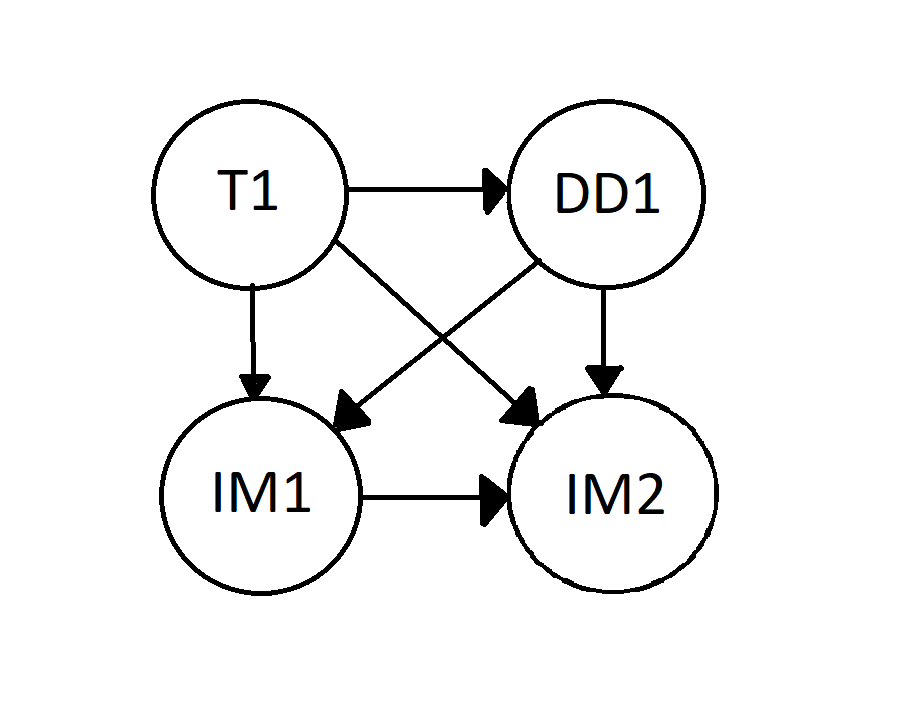
\includegraphics[width=\textwidth]{ATrace.png}
%		}
%		\caption{\label{Fig_ATrace} Traceability Matrix Showing the Connections 
%		Between Items of Different Sections}
 %	\end{center}
% \end{figure}

 %\begin{figure}[h!]
%	\begin{center}
%		%\rotatebox{-90}
 %		{
%			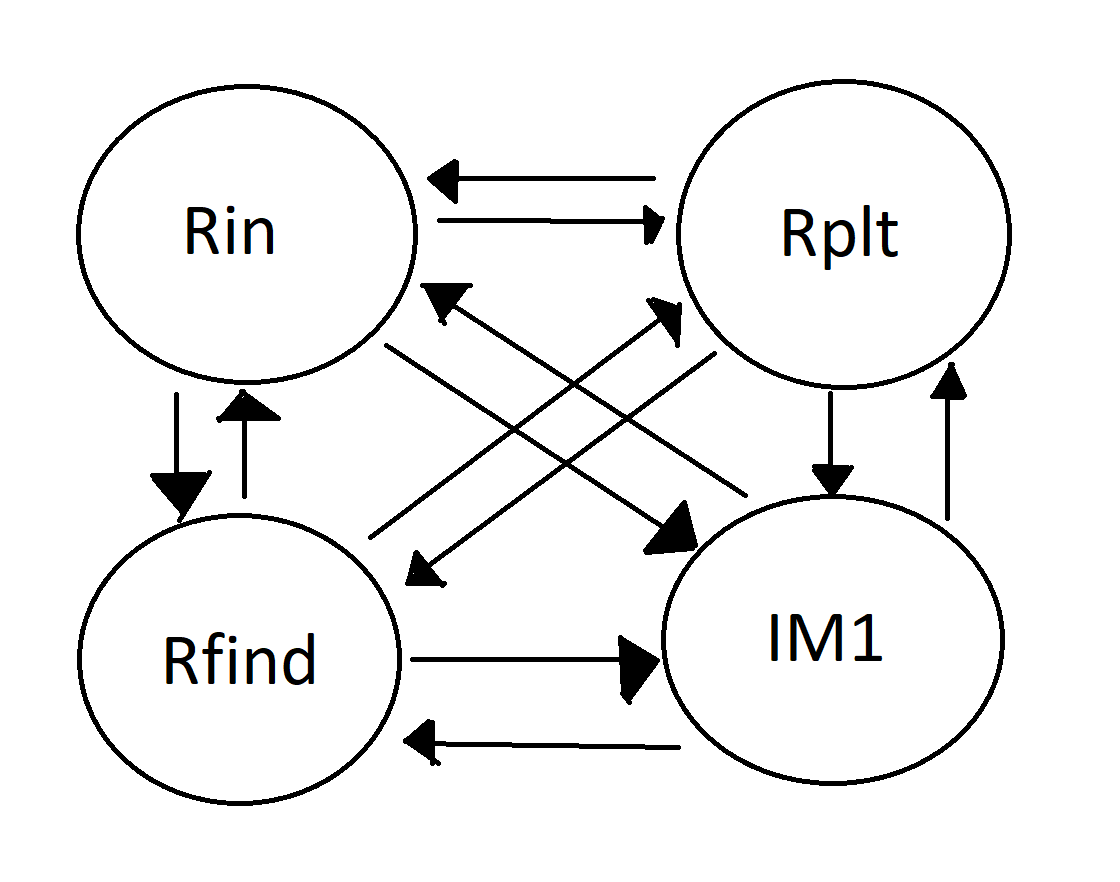
\includegraphics[width=0.7\textwidth]{RTrace.png}
%		}
 %%		Between Requirements, Instance Models, and Data Constraints}
%	\end{center}
 %\end{figure}

\newpage

\bibliographystyle {plainnat}
\bibliography {../../ReferenceMaterial/References}

\newpage

\section{Appendix}

\wss{Your report may require an appendix.  For instance, this is a good point to
show the values of the symbolic parameters introduced in the report.}

\subsection{Symbolic Parameters}

\wss{The definition of the requirements will likely call for SYMBOLIC\_CONSTANTS.
Their values are defined in this section for easy maintenance.}

\end{document}